\documentclass[10pt,a4paper]{article}
\usepackage[english]{babel}
\usepackage{multicol}
\usepackage{multirow}
\usepackage{url,hyperref,graphicx,float,times}
\usepackage{sectsty}
\usepackage{authblk}
\usepackage{textcomp}
\renewcommand{\refname}{}

\setlength{\paperheight}{297mm}
\setlength{\paperwidth}{210mm}
\setlength{\voffset}{-12mm}
\setlength{\topmargin}{0mm}
\setlength{\headsep}{8mm}
\setlength{\headheight}{10mm}
\setlength{\textheight}{235mm}
\setlength{\hoffset}{-4mm}
\setlength{\textwidth}{166mm}
\setlength{\oddsidemargin}{0mm}
\setlength{\evensidemargin}{0mm}
\setlength{\marginparwidth}{0mm}
\setlength{\marginparpush}{0mm}
\setlength{\columnsep}{6mm}
\setlength{\parindent}{6mm}
\setlength{\parskip}{2mm}

%% insert eps pictures
%% use as \epsin{epsfile}{width_in_mm}{label}{caption}
\usepackage{epsfig}
\newcounter{figcounter}
\def\epsin #1#2#3#4{
\refstepcounter{figcounter} \label{#3}
\[
\mbox{
  \epsfxsize=#2mm
  \epsffile{#1.eps}
}
\]
%\vspace{0mm}
\begin{center}
  \parbox{7cm}{{\bf FIGURE \arabic{figcounter}:}\quad {\it #4 } } \\
\end{center}
}

%% insert table
%% use as \tabin{size_in_mm}{label}{caption}{table_data}
\newcounter{tabcounter}
\def\tabin #1#2#3#4{
\refstepcounter{tabcounter} \label{#2}
\[ \makebox[#1mm][c]{#4} \]
%\vspace{0mm}
\begin{center}
  \parbox{7cm}{{\bf TABLE \arabic{tabcounter}:}\quad {\it #3 } } \\
\end{center}
}

\title{\LARGE
Performance Evaluation of Xenomai 3
}

\author[*]{\large
{\bf Ching-Chun (Jim) Huang}\thanks{jserv@ccns.ncku.edu.tw}}
\author[**]{\large
{\bf Chan-Hsiang Lin}\thanks{r04943031$@$ntu.edu.tw}}
\author[*]{\large
{\bf Che-Kang Wu}\thanks{an4006048$@$mail.ncku.edu.tw}}
\affil[*]{Department of Computer Science and Information Engineering,
\newline
National Cheng Kung University, Taiwan
\newline
No.1, University Road, Tainan City 701, Taiwan (R.O.C.)}
\affil[**]{Department of Electrical and Electronic Engineering,
\newline
National Taiwan University
\newline
No.1, Sec. 4, Roosevelt Road, Taipei, Taiwan (R.O.C.)}
\date{}


\begin{document}

\maketitle

\begin{abstract}
Xenomai 3 is the new architecture of the real-time framework running seamlessly side-by-side Linux as a dual-kernel system like Xenomai 2, or natively over mainline Linux kernels supplemented by the PREEMPT\_RT efforts to meet stricter response time requirements than standard kernel preemption would bring. In this presentation, we will evaluate the performances of Xenomai 3 running with dual-kernel configuration and analyze the various benchmarks for ARM Cortex-A series. Xenomai 3 introduces some optimizations over RTOS API emulation, thread-to-thread communications, and significantly lower overhead with dual-kernel configurations. The comprehensive performance comparisons illustrate the major evolution of Xenomai 3 along with the revised Real-Time Driver Model (RTDM) which provides a unified interface over both PREEMPT\_RT and dual-kernel.

This paper would be a report on performance measurements between upstream Linux real-time enhancements and Xenomai official stable release (both version 2 and 3 series), and the benchmarks show that the maximum response time to external interrupts of the dual kernel configurations for Xenomai 3 is still better than PPREEMPT\_RT, that implies more predictable handling on multiple incoming interrupts where Xenomai 3 supports both configurations interchangeably.
\end{abstract}

\vspace{10mm}

\begin{multicols}{2}

\section{Introduction}
The default Linux is designed to optimize for total system throughput, rather than for interactivity or the ability to perform real-time work. Historically speaking, there are two typical approaches to modifying the standard Linux kernel into a real-time kernel. The first introduces an extra small real-time executive \cite{rtai} or microkernel \cite{sel4} which runs the modified Linux kernel as a task. The small real-time executive, sometimes referred to \textit{co-kernel}, takes control over the system for real-time processes and is responsible for scheduling real-time tasks, interrupt handling and scheduling Linux. With these changes it is possible to let a real-time task run on the CPU without the Linux kernel being able to interrupt the task. As the Linux kernel is run as a task it is preemptive at any time.

Another approach is to make the Linux kernel itself more real-time by reducing the durations for which high-priority operations can be blocked, at the cost of reducing overall throughput. \textit{PREEMPT\_RT} \cite{linux-rt}, maintained separately from the Linux upstream, results in pure kernel implementation, and neither application programming interface (API) nor application binary interface (ABI) change is required. PREEMPT\_RT allows the use of existing Linux device drivers from real-time applications by making many spinlock-guarded regions preemptible, moving IRQ handlers into threads, and adding various other real-time features.

In this section we briefly present the Xenomai \cite{xenomai} real-time framework for Linux, and its base real-time executive, Adaptive Domain Environment for Operating System (Adeos) nanokernel \cite{adeos}, which allows Xenomai and Linux to run on the same hardware.

\subsection{Adeos nanokernel}

\textit{Adeos} is a resource virtualization layer, allowing multiple entities called \textit{domains}, which can compete with each other for receiving system generated \textit{events}. Those events can be incoming external (or virtually generated) interruptions, Linux system calls invocations, or various kernel-code-related events like context switches. Adeos introduces the \textit{event pipeline}, which can be seen as a chain of domains of decreasing priority. The events are consequently propagated throughout the pipeline, distributed firstly to the utmost priority domain, then distributed to lower priority domains.

Adeos is maintained by its I-pipe software. In Xenomai parlance, the I-pipe and Adeos both refer to the almost same code, that makes a Linux kernel able to host a secondary kernel exhibiting real-time properties (e.g. Xenomai), on the same hardware. I-pipe is a kernel patch applied to a regular Linux kernel, which among other services, guarantees delivery of external interrupts to Xenomai with very low latency. However, since Xenomai 3 supports PREEMPT\_RT, I-pipe is dependant only for running Xenomai in a dual kernel configuration.

\subsection{Xenomai}

Xenomai provides a kernel-based API for real-time applications. A user-space API is also available, at the cost of longer latencies. Xenomai introduces the concept of \textit{skins} \cite{ChameleonRTOS}, emulating proprietary APIs used for migrating real-time applications from various RTOSs like \textit{VxWorks}, \textit{pSOS}, \textit{VRTX}, etc. to Xenomai.

All Xenomai skins rely on the common the core of the RTOS, implementing all algorithms for real-time functionalities. Xenomai 3 provides all standard services one can expect to find in a classical RTOS such as handling interrupts and scheduling real-time threads, by means of two options: Cobalt and Mercury.

\subsection{Cobalt}

\textit{Cobalt}, distinguished in Xenomai 3, is the real-time extension, built into the Linux kernel, dealing with all time-critical activities on top of Adeos I-pipe. The Cobalt core has higher priority over the native kernel activities and has the same behaviour as what Xenomai 2 delivers real-time. For both Cobalt (as known as \textit{dual kernel} configurationin Xenomai 3) and Xenomai 2, the Linux kernel receives only virtual interrupt events, and those only after higher-priority software (e.g. the Xenomai layer) has had an opportunity to respond first. Similarly, when the Linux kernel blocks interrupt handlers, it does so only for itself; high-priority Xenomai threads will receive their events from the I-pipe on schedule.

In the dual kernel configuration of Xenomai 3, all the RTOS APIs Xenomai provides interface with the Cobalt core, and only those APIs are deemed real-time capable, including the subset of POSIX 1003.1c \cite{posix-1003-1c} services implemented by \textit{libcobalt}, which was named after \textit{nucleus} in Xenomai 2.

\begin{figure}[H]
\begin{center}
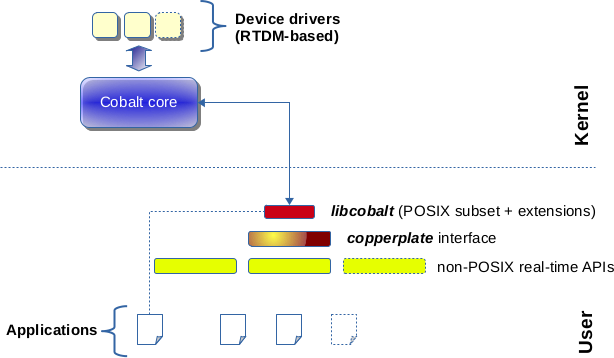
\includegraphics[width=8cm]{img/x3-cobalt.png}
\caption{Xenomai 3 dual kernel configuration}
\label{xenomai3-coblat}
\end{center}
\end{figure}


\subsection{Mercury}

\textit{Mercury} was derived on the past experiment, \textit{Xenomai/SOLO} project \cite{xenomai-solo}, as an intermediate step towards Xenomai 3. Xenomai/SOLO project was the clean-room re-implementation of the building blocks that connect an emulator with the underlaying RTOS with special respect to the requirements and semantics of the native Linux kernel. The VxWorks emulator was the first one built over the Xenomai/SOLO project, as proof of concept (PoC), providing the VxWorks core API that can be used to port existing VxWorks applications to native Linux.

Xenomai 2 provides skins to emulate traditional RTOS, such as VxWorks and pSOS, and a number of projects have been migrated smoothly from one of the supported traditional RTOS to Xenomai. In order to use a similar approach to migrate traditional RTOS projects to native Linux as well, Xenomai 3.x was launched. Thus, the single kernel configuration, Mercury, in Xenomai 3 does rely on the real-time capabilities of the native Linux kernel. Often, applications will require the PREEMPT\_RT extension to be enabled in the target kernel, for delivering real-time services.

PREEMPT\_RT is not mandatory, however, and Mercury depends on the application requirements with respect to responsiveness and maximum jitter; some may even tolerate a certain percentage of deadline misses.

In this single kernel configuration, all the non-POSIX RTOS APIs Xenomai provides are accurately emulated over the native threading library (preferably NPTL).

\begin{figure}[H]
\begin{center}
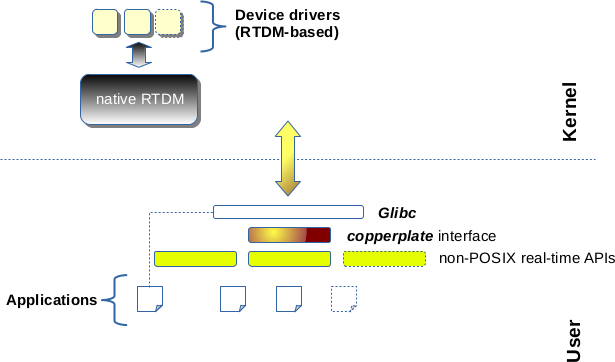
\includegraphics[width=8cm]{img/x3-mercury.png}
\caption{Xenomai 3 single kernel configuration}
\label{xenomai3-coblat}
\end{center}
\end{figure}

Xenomai 3 offers both dual-kernel and native option, and it deploys same Alchemy \cite{x3-applications} API on Cobalt/I-pipe and PREEMPT\_RT. Xenomai 3 was designed for tight latency requirement, configuration flexibility, and system compatibility.

\section{Measurement system design}
There are two objectives for performance evaluations. First, comparing the performance of Xenomai with mainline Linux kernel and PREEMPT\_RT to exploit the real-time capability from system view. Second, trying to quantize the performance improvements and potential degradation of Xenomai 3.

\subsubsection{Hardware}
\textit{BeagleBone Black}\cite{bbb} is selected as our major testing hardware platform powered by \textit{TI AM335x} \cite{am335x}, and it is an effective embedded platform, capable of running Linux and Xenomai (both 2 and 3), consisting of a single 1GHz ARM Cortex-A8 processor, a 512 MB memory, 32kB L1 caches and a 256kB L2 cache.

Beaglebone Black is community-supported development platform, and active Linux kernel maintenance enables us to perform further experiments and participate in technical discussions. TI AM335x is used widely in industrial automation, providing an extensive, reliable solution portfolio ranging from robust microcontrollers to ARM based microprocessors.

\subsubsection{Software Installation}
Debian GNU/Linux image 2014-05-14 \cite{debian} was installed on the BeagleBone Black, with hardware-specific Linux kernel tree from official BeagleBone kernel repository \cite{kernel}. We selected kernel version 3.14.39 due to its compatibility with all kernel configurations after our early evaluations.

Four distinct Linux kernel configurations are used for the experiments, as summarized in table below. Kernel are patched using git merge first, and remaining conflicts are resolved manually.

The kernel configuration options are mostly following the default. However, some of the default configuration may have an impact on real-time latencies, such as the ones about CPU Power Management, APM support, and opportunistic sleep. Additionally, most debugging facilities in Kernel hacking section lead to increased latencies. Those problematic options are disabled manually during the whole experiments.

\begin{tabular}{|l| p{3cm} |l|}
\hline
Kernel & Patches & Source\\ \hline
mainline   & N/A & N/A \\ \hline
PREEMPT\_RT & patch-3.14.39-rt37 & \cite{p-rt} \\ \hline
Xenomai 2  & ipipe-core-3.14.39-arm-9 + xenomai v2.6.4 (Jul 13, 2015; HEAD) & \cite{p-ipipe} \cite{git-x2.6} \\ \hline
Xenomai 3  & ipipe-core-3.14.39-arm-9 + xenomai v3.0 (Oct 8, 2015) & \cite{p-ipipe} \cite{git-x3} \\ \hline
\end{tabular}\\
\vspace{4mm} \\
Table 1: Different kernel configurations for the experiment\\

\subsubsection{Prerequisites for Experiments}
We tried to measure the latencies under 2 conditions: IDLE and CPU-STRESSED. In the IDLE condition, in order to create such test environment, some non-essential user processes were eliminated. While in the CPU-STRESSED condition, these process are also forcely killed, and we used the \textit{stress} \cite{stress} utility to keep the CPU busy. The commands to kill these processes are written in the test script.

  The gravity values is the shortest time the platform needs to deliver an IRQ to a Xenomai interrupt handler, a RTDM task running in kernel space, or a user-space task. It is used to differentiate timers on the target context they activate, among IRQ (handlers), kernel and user threads, anticipating the next timer shot accordingly, so that such context is activated as close as possible to the ideal time. The gravity values can be set in the file \begin{verbatim}/proc/xenomai/latency
\end{verbatim} on Xenomai 2, and in the file
\begin{verbatim}/proc/xenomai/clock/coreclk
\end{verbatim} on Xenomai 3 with root privilege. Furthermore, Xenomai 3 provides an \textit{autotune} tool running a series of internal calibration tests for estimating the most appropriate gravity values for its real-time clock timer, retaining the final values.

Because Xenomai 2 does not provide the corresponding autotune tool, and it has only one gravity value for all the coreclocks, we decided to manually tune all the coreclock values in both Xenomai 2 and Xenomai 3 to zero, so that we can compare the results on the same basis later

In our experiments, the kernel build were persistent in different SD/MMC media. The fact that different external storage devices have different access speeds could affect the final results. In order to eliminate the uncertainties and prevent the test process' pages from being swapped into disk, we locked all the test processes' pages inside memory. While using \textit{cyclictest} tool, we can achieve by specifying the '-m' option along with the command. On the other hand, we exclude the known latency factors and execute programs within the memory-locked environment.

\subsection{Performance Evaluation}

\subsubsection{Test scenario}
We prepared comprehensive statistics collection for the real-time performance results of mainline Linux kernel, PREEMPT\_RT, Xenomai 2 and Xenomai 3. In addition, we expect to figure out the performance benefits from the newly released Xenomai version 3.0, the first official release of Xenomai 3, comparing to Xenomai-2.6.4, the latest stable release of Xenomai 2. This new architecture of Xenomai 3 exhibits two real-time options, selected at build time. The dual kernel configuration of Xenomai 3, Cobalt, is a significant rework of the Xenomai 2 system. And, the single kernel natively over mainline Linux kernels, which can be supplemented by the PREEMPT\_RT to meet stricter response time requirements.

Since the single kernel configuration is built upon mainline kernel or PREEMPT\_RT, we do not have to measure its configuration separately because of the availability of PREEMPT\_RT in our benchmark matrix.

In Xenomai 3, with the introduction of the \textit{Copperplate} interface, which mediates between the real-time API / emulator of given application uses, and the underlying real-time core. That is, applications are able to run in either environments without visible code change. 

The default interfaces have switched to being POSIX-based (Copperplate library) in Xenomai 3, so all other real-time APIs (or skins) are implemented on top of this. In particular, the Xenomai 2 native API (now called Alchemy) is a skin, while the POSIX API has been promoted from a skin to the standard interface. We do not intend to measure the overhead of \textit{Copperplate} interface or its implementation for the sake of measuring the system-level performance rather than API-oriented emulation.

\subsubsection{Performance Tools}
\textit{Cyclictest}, maintained in \textit{rt-tests} \cite{rt-tests} package, is a commonly-used latency benchmark. It is compatible with all of the kernel setups we use (the recently Xenomai 3.0 release shipped with cyclictest in its testsuite), therefore it is suitable for the purpose of measuring latencies for all setups.

\textit{Latency} is a test program provided by the Xenomai test suite (available in both Xenomai 2 and 3). It can measure latencies under 3 modes: \textit{user task}, \textit{kernel task}, or \textit{timer IRQ}. It launches the test procedure in one of the user-specified contexts. In the user mode, the measurement task is handled by the 'latency' function in the program, which periodically waits and fetches the current time when resuming. Latency is then measured by calculating the difference of the actual time elapsed with the predefined period.

\subsubsection{Test Procedure}
Each experiment was run on the same Beaglebone Black hardware device. Each was run for 20 minutes to generate approximately 1,000,000 samples. Test scripts were written to facilitate the experiment process.

\subsubsection{Test Load}
As previously mentioned, we measure latencies under IDLE and CPU-STRESSED conditions. In the CPU-STRESSED condition, we invoked the "stress" process to exert pressure on the CPU.

\subsection{Experiment Result}
\begin{figure}[H]
\begin{center}
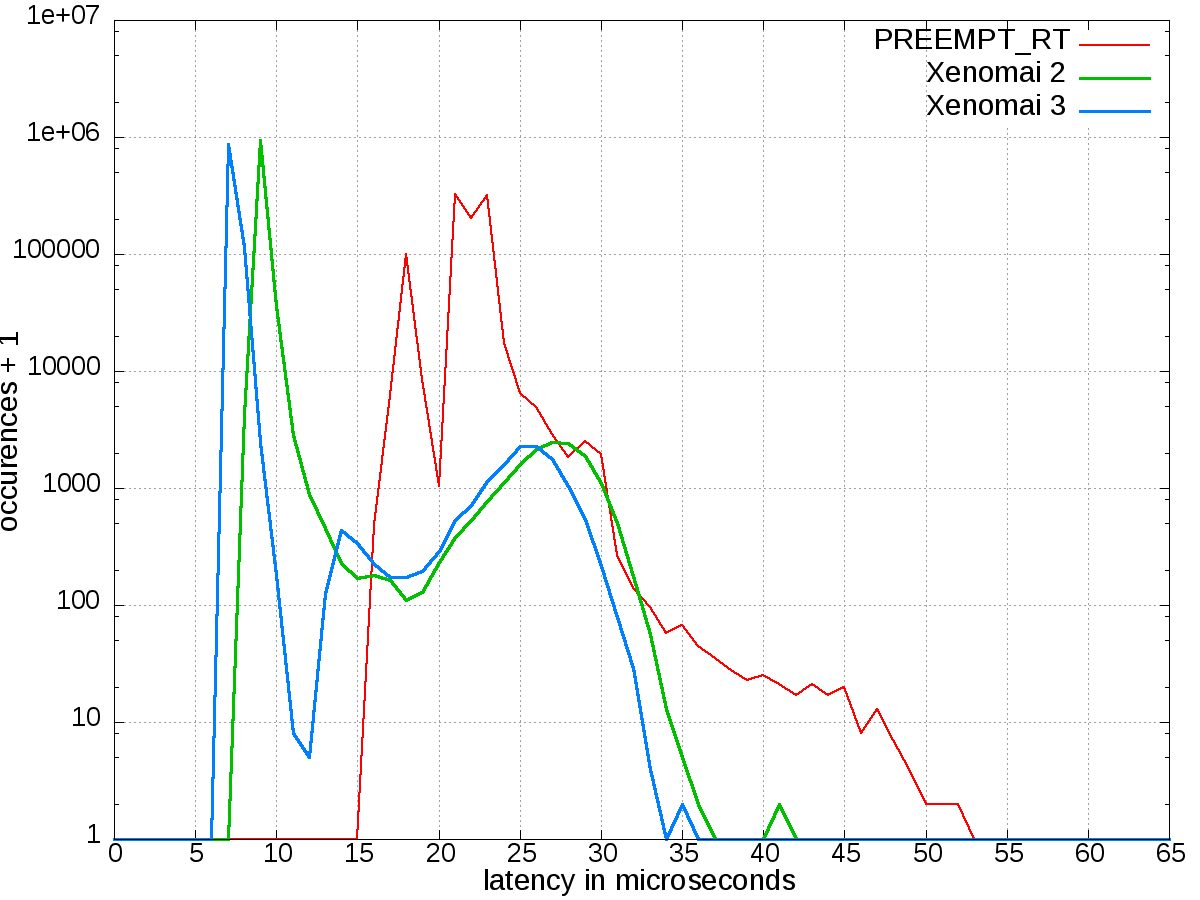
\includegraphics[width=6cm]{img/cyclictest_idle.jpg}
\caption{Cyclictest with no stress.}
\label{cyclictest-idle}
\end{center}
\end{figure}
%%%%%%%%%%%%%%%%%%%%%%%%%
\begin{figure}[H]
\begin{center}
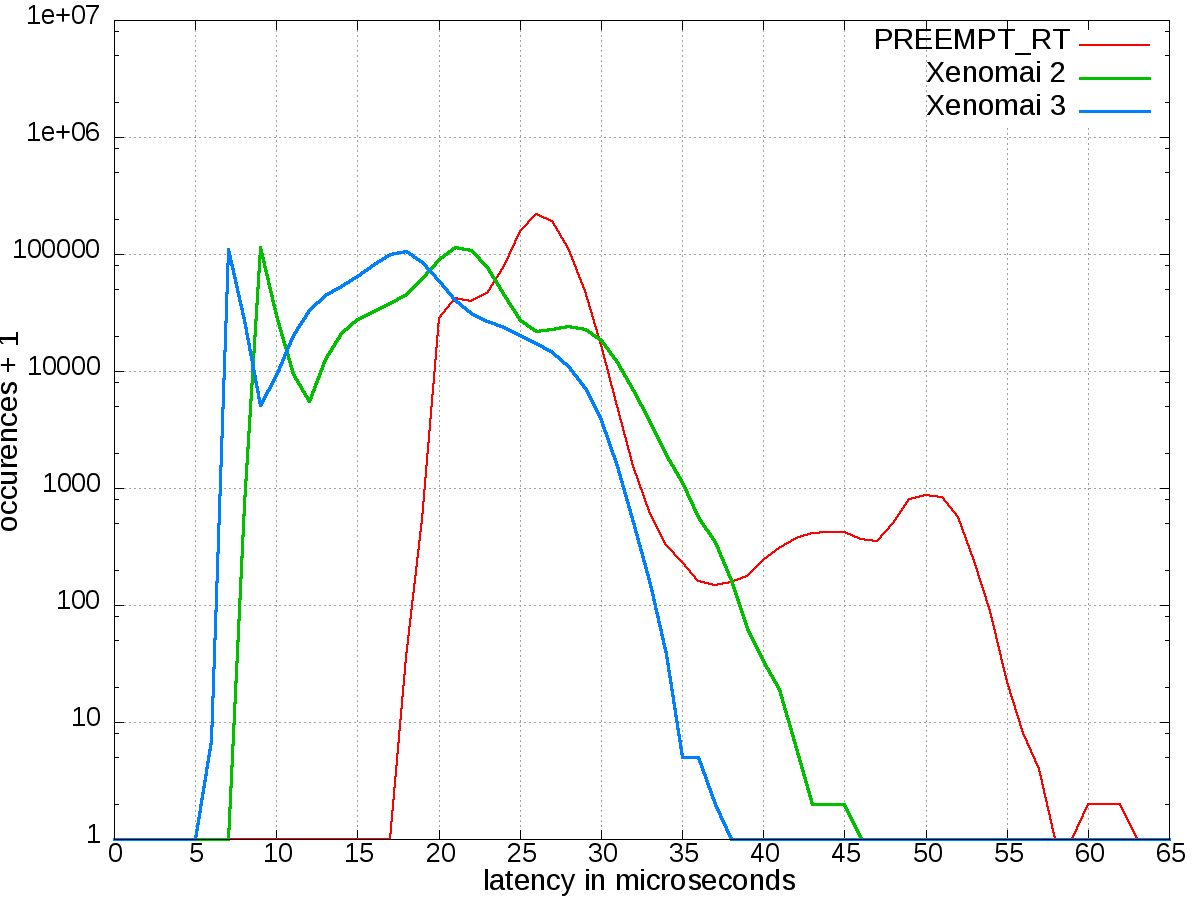
\includegraphics[width=6cm]{img/cyclictest_stress.jpg}
\caption{Cyclictest with stress.}
\label{cyclictest-stress}
\end{center}
\end{figure}
%%%%%%%%%%%%%%%%%%%%%%%%%
\begin{figure}[H]
\begin{center}
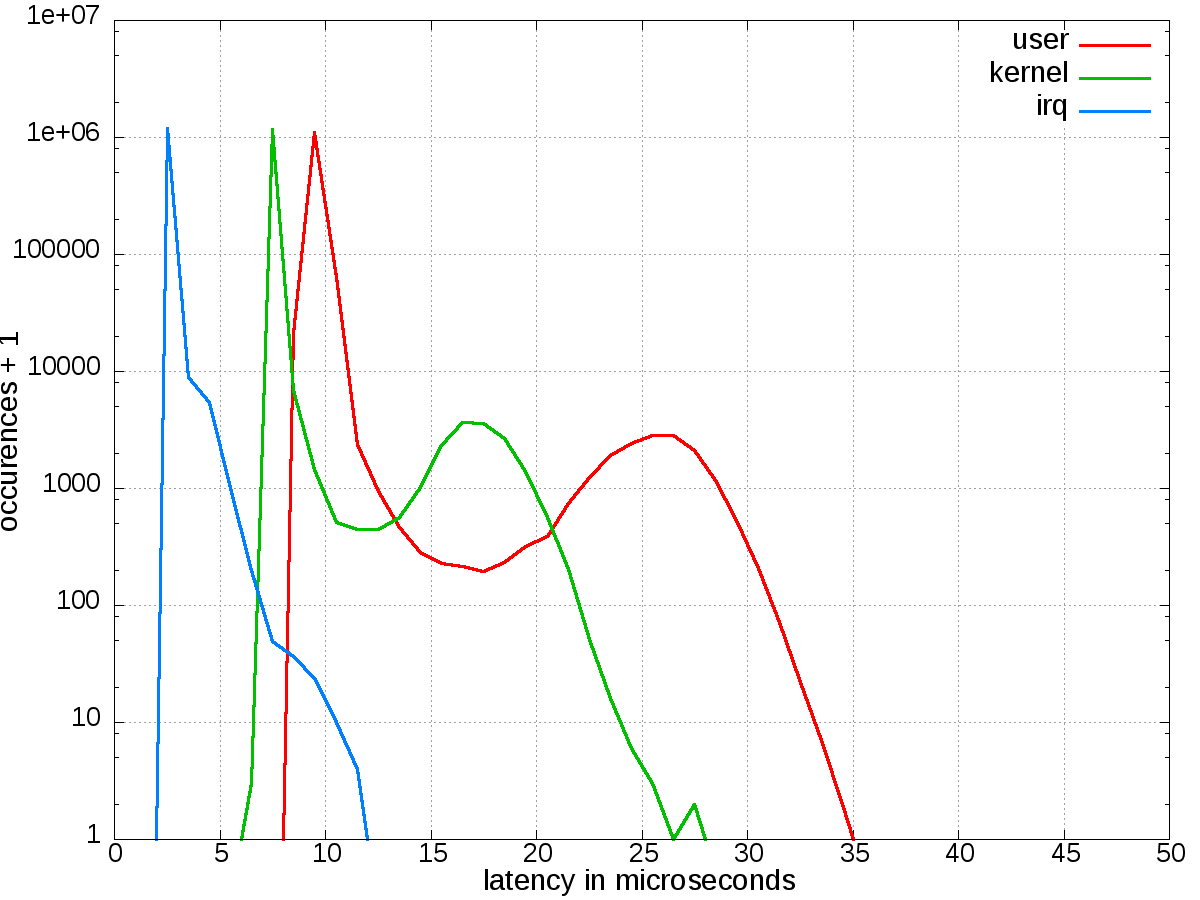
\includegraphics[width=6cm]{img/x2-idle.png}
\caption{Latency with no stress on Xenomai-2.}
\label{x2-latency-idle}
\end{center}
\end{figure}
%%%%%%%%%%%%%%%%%%%%%%%%%
\begin{figure}[H]
\begin{center}
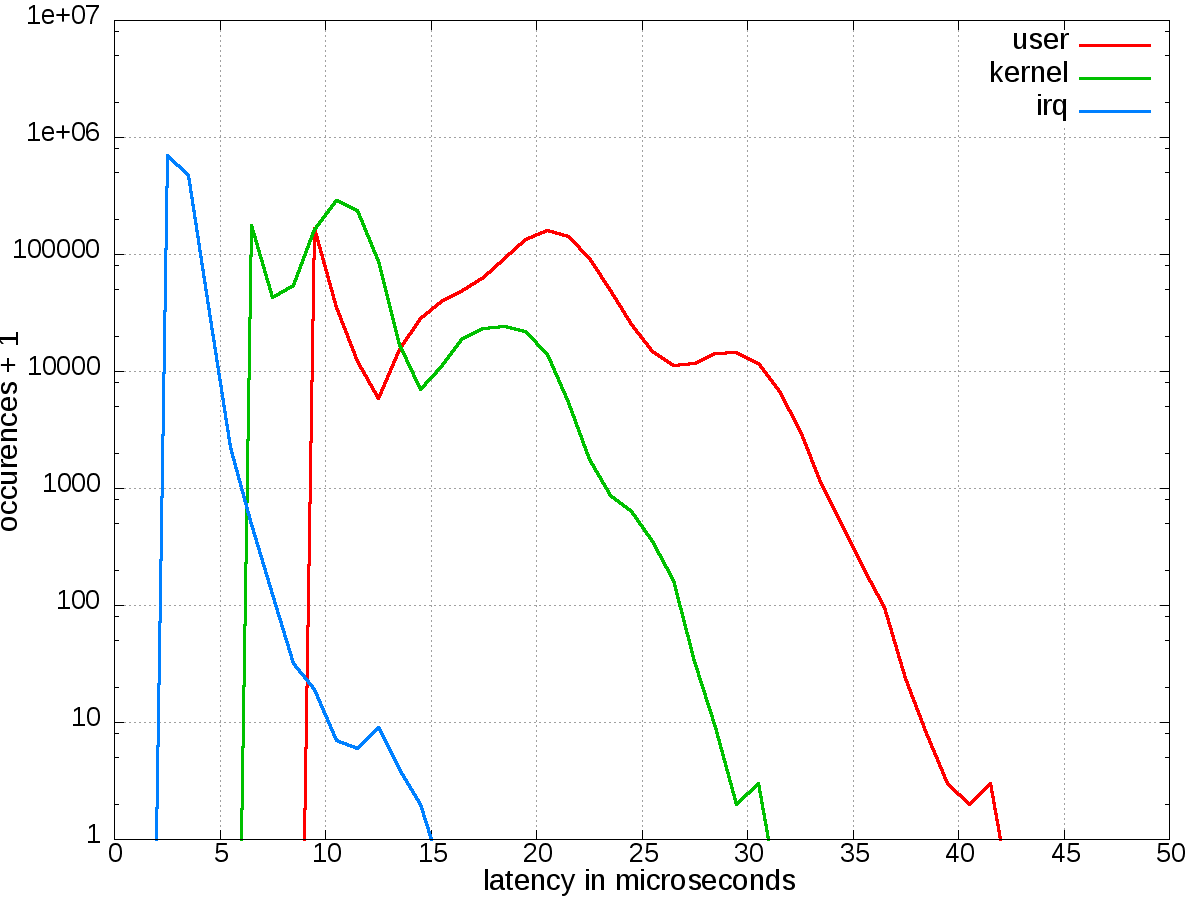
\includegraphics[width=6cm]{img/x2-cpu.png}
\caption{Latency with stress on Xenomai-2.}
\label{x2-latency-stress}
\end{center}
\end{figure}
%%%%%%%%%%%%%%%%%%%%%%%%%
\begin{figure}[H]
\begin{center}
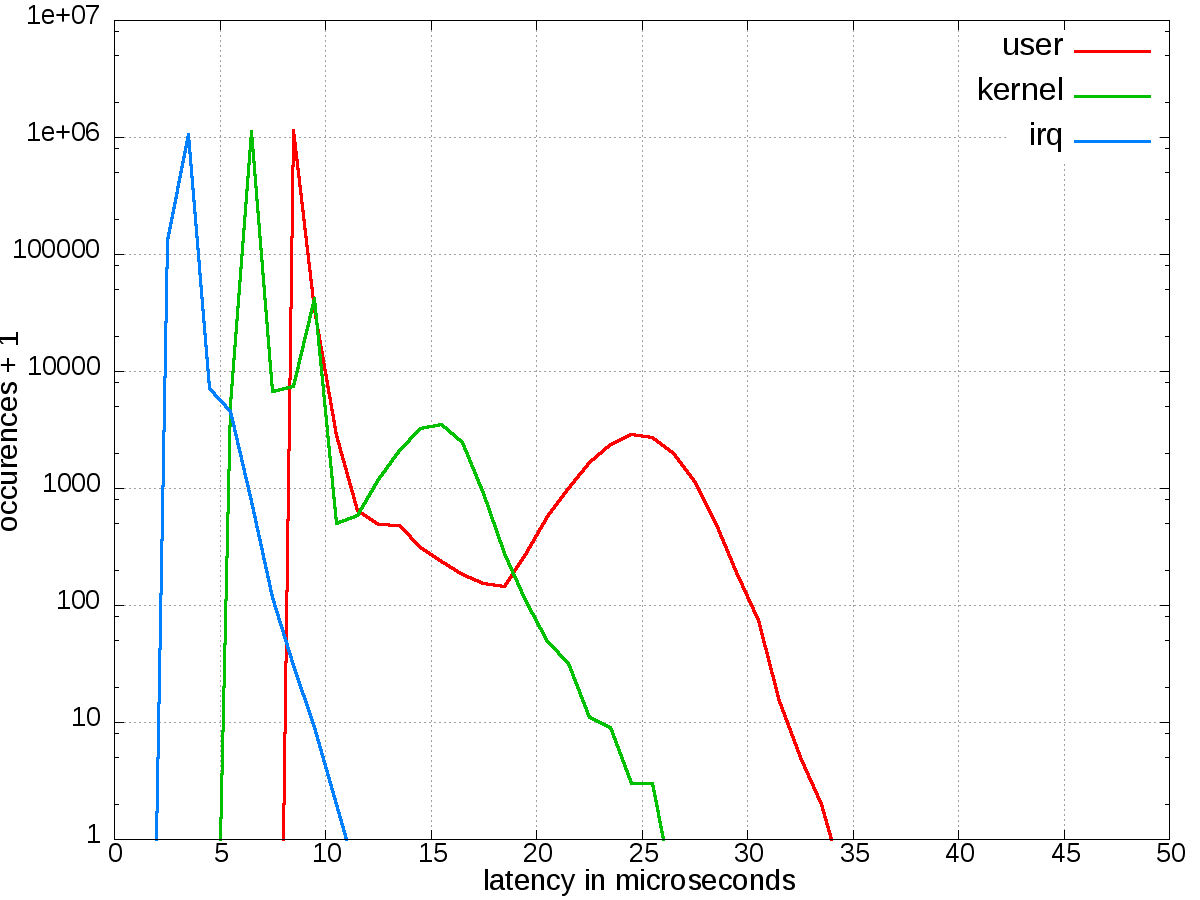
\includegraphics[width=6cm]{img/x3-idle.png}
\caption{Latency with no stress on Xenomai-3.}
\label{x3-latency-idle}
\end{center}
\end{figure}
%%%%%%%%%%%%%%%%%%%%%%%%%
\begin{figure}[H]
\begin{center}
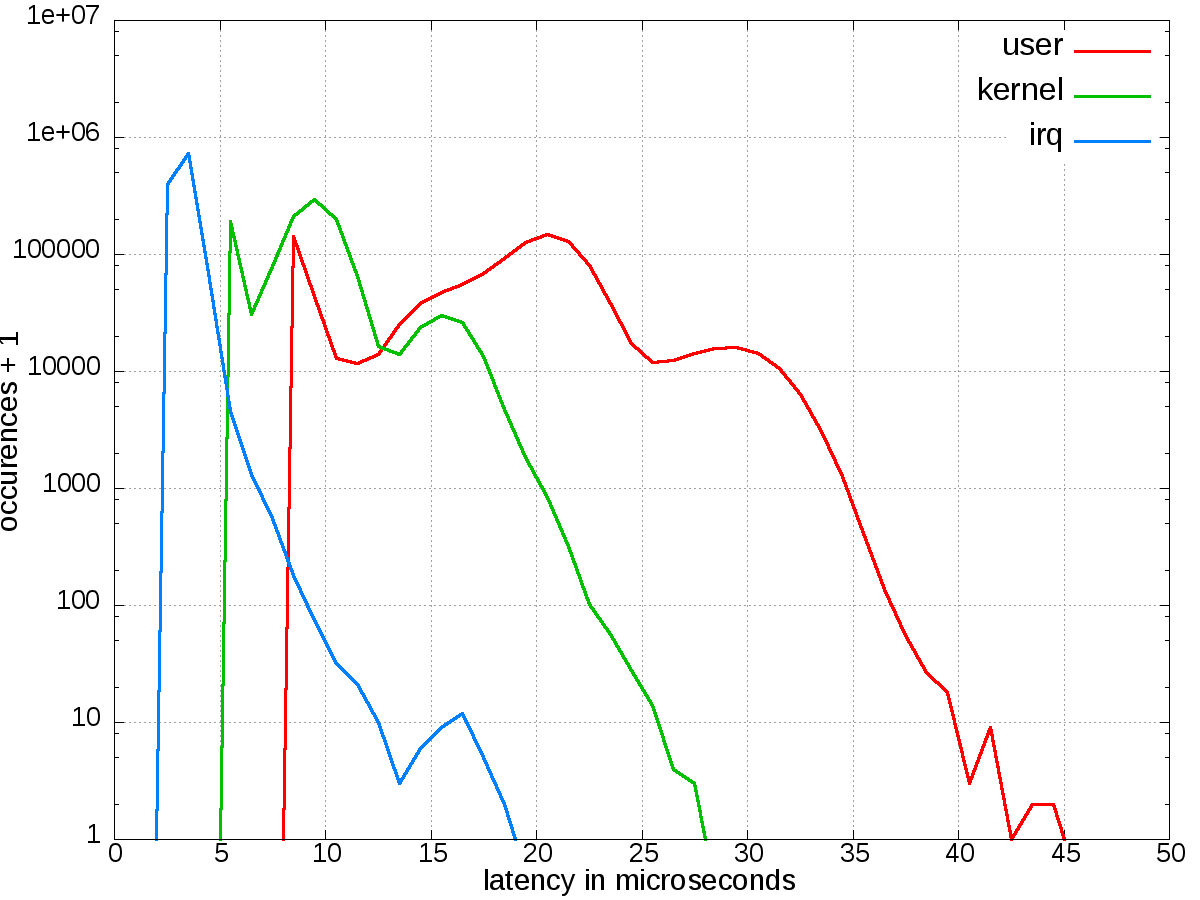
\includegraphics[width=6cm]{img/x3-cpu.png}
\caption{Latency with stress on Xenomai-3.}
\label{x3-latency-stress}
\end{center}
\end{figure} 
%%%%%%%%%%%%%%%%%%%%%%%%%
\begin{tabular}{|l|r|r|r|}
\hline
\multirow{2}{*}{} & \multicolumn{3}{c|}{idle}  \\ \cline{2-4} 
 & \multicolumn{1}{l|}{min} & \multicolumn{1}{l|}{avg} & \multicolumn{1}{l|}{max} \\ \hline
Mainline Linux & 39 & 43 & 1046  \\ \hline
Preempt-RT & 16 & 21 & 52 \\ \hline
Xenomai 2 & 8 & 9 & 41 \\ \hline
Xenomai 3 & 7 & 7 & 35 \\ \hline
 & \multicolumn{3}{c|}{cpu-stressed} \\ \hline
Mainline Linux & 39 & 52 & 1097 \\ \hline
Preempt-RT & 18 & 25 & 62 \\ \hline
Xenomai 2 & 8 & 19 & 45 \\ \hline
Xenomai 3 & 6 & 16 & 37 \\ \hline
\end{tabular}\\
\vspace{4mm} \\
Table 2: cyclictest result on different kernel setups, in \textmu s\\
\vspace{4mm} \\
%%%%%%%%%%%%%%%%%%%%%%%%%
\begin{tabular}{|l|c|r|r|}
\hline
\multirow{2}{*}{} & \multicolumn{3}{c|}{user} \\ \cline{2-4} 
 & min & \multicolumn{1}{c|}{avg} & \multicolumn{1}{c|}{max} \\ \hline
Xenomai 2 & 8.541 & 9.458 & 34.583 \\ \hline
Xenomai 3 & 8.043 & 8.853 & 33.023 \\ \hline
& \multicolumn{3}{c|}{kernel}      \\ \hline
Xenomai 2 & 6.965 & 7.708 & 27.821 \\ \hline
Xenomai 3 & 5.567 & 6.479 & 25.577 \\ \hline
& \multicolumn{3}{c|}{timer-irq}   \\ \hline
Xenomai 2 & 2.129 & 2.654 & 11.343 \\ \hline
Xenomai 3 & 2.586 & 3.079 & 10.031 \\ \hline
\end{tabular} \\
\vspace{4mm} \\
Table 3: latency result on different kernel setups, in \textmu s\\

From the data above, it shows that the latency performance of timer-irq in CPU-STRESSED situation is slightly worse on Xenomai-3(over 3 us) than on Xenomai-2(below 3 us). While this is not an occasional case(the same experiment was ran a couple of times), we tried to look into the test code of latency to figure out the cause of this phenomenon. In user-level mode, the measurement task is carried out by the function 'latency' inside the program; whereas in kernel or irq mode, the task is executed by issuing a Xenomai RTDM command such as 
\begin{verbatim}
rt_dev_ioctl(benchdev, \
RTTST_RTIOC_INTERM_BENCH_RES,&result); 
\end{verbatim} 
in an infinite loop to periodically launch timer and capture latencies. Unfortunately, we were unable to discover the reason for the discrepancy on the observed data.
\subsection{Experiment Result Analysis}
Our data shows that the average user-level latency in either Xenomai 2 or 3 is around 9 \textmu s in idle condition, 18 \textmu s in stressed condition. And in the worse case, the latency is below 50 \textmu s. Meanwhile, the latency of PREEMPT\_RT has an averaged user-level latency more than 20 \textmu s, which means it can not guarantee a 50 \textmu s max latency (Actually in some cases the latency will exceed 100 \textmu s in stressed condition).  As for mainline Linux, the max latency easily exceeds 1 ms. When comparing the performance of Xenomai 3 to Xenomai 2, we can see that the statistics in cyclictest and latency test is slightly better, except for the case of timer-irq latency in stressed condition.

\section{Conclusions}
We have evaluated the performance of two approaches to make Linux being real-time: PREEMPT\_RT and Xenomai, diversely presented in the view of single kernel and dual-kernel configurations on single-core ARM Cortex-A8, along with general conclusions about when each kernel configuration. As for the dual kernel configuration of Xenomai 3, latency is still significantly better, but PREEMPT\_RT shows closer performance at least for Linux kernel 3.14 stable release while it enables to run same application on different platforms and migrate existing POSIX application to Linux systems.

The Linux kernel running under Xenomai 3 can be PREEMPT\_RT as well through the native option of Xenomai 3 for maximum API/ABI compatibility in real-time environments. For the tight latency requirements such as real-time networking, Xenomai 3 allows to switch to dual kernel configurations utilizing I-pipe for maximum real-time performance, which brings sligtly better performance than Xenomai 2. However, comparing to Xenomai 2, our results show the unexpected slowdown of timer irq latency in stressed condition while Xenomai 3 was configured as the dual kernel configuration.


\bibliographystyle{unsrt}
\begin{thebibliography}{9}%use this if you have <=9 bib refs
	\bibitem {rtai}{\it https://www.rtai.org/}
	\bibitem {sel4}{\it http://ssrg.nicta.com.au/projects/seL4/}
	\bibitem {linux-rt}{\it http://git.kernel.org/cgit/linux/kernel/git/rt/}
	\bibitem {xenomai}{\it http://xenomai.org/}
	\bibitem {adeos} Karim Yaghmour. Adaptive Domain Environment for Operating Systems.\\
	    \url{http://www.opersys.com/ftp/pub/Adeos/adeos.pdf}
	\bibitem {ChameleonRTOS}{\it http://www.xenomai.org/documentation/slides/Xenomai-OSMB-2007-01.pdf}
	\bibitem {posix-1003-1c}{\it http://standards.ieee.org/findstds/interps/1003-1c-95\_int/}
	\bibitem {xenomai-solo}{\it https://www.osadl.org/Xenomai-SOLO.xenomai-solo.0.html}
	\bibitem {x3-applications}{\it http://xenomai.org/running-applications-with-xenomai-3-x/}
	\bibitem {bbb}{\it http://beagleboard.org/BLACK}
	\bibitem {am335x}{\it http://www.ti.com/lsds/ti/processors/sitara/arm\_cortex-a8/am335x/overview.page}
	\bibitem {debian}{\it http://debian.beagleboard.org/images/bone-debian-7.5-2014-05-14-2gb.img.xz}
	\bibitem {kernel}{\it https://github.com/beagleboard/linux}
	\bibitem {p-rt}{\it https://www.kernel.org/pub/linux/kernel/projects/rt/3.14/}
	\bibitem {p-ipipe}{\it http://download.gna.org/adeos/patches/v3.x/arm/ipipe-core-3.14.39-arm-9.patch}
	\bibitem {git-x2.6}{\it http://git.xenomai.org/xenomai-2.6.git/}
	\bibitem {git-x3}{\it http://git.xenomai.org/xenomai-3.git/}
	\bibitem {stress}{\it http://people.seas.harvard.edu/~apw/stress/}
	\bibitem {rt-tests}{\it https://rt.wiki.kernel.org/index.php/Cyclictest}
\end{thebibliography}

\end{multicols}
\end{document}
